\section{Wstęp}
%%%%%%%%%%%%%%%%
\begin{frame}{Wstęp}
    Szukamy pierwiastków równań typu
    \[
    f(x) = 0 \quad \textrm{(1 zmienna)}
    \]
    \begin{tabbing}
	    $f(x)$:\quad \= - o wartościach rzeczywistych\\
	    \> - ciągła
    \end{tabbing}
	{\bf Pierwiastek} - liczba $\alpha : f(\alpha) = 0$
	\begin{tabbing}
		Np:\\
		\quad 1. $e^{-x} - \sin(x) = 0$\\
		\quad 2. $x^{3} - 3x + 1 = 0 \quad\rightarrow\quad$ zera wielomianu (przypadek szczególny)
	\end{tabbing}
	{\bf Istota} - znajomości $f(x)$: papier, ołówek, kalkulator! - warto na początku!
\end{frame}
%%%%%%%%%%%%%%%%
\begin{frame}{Wstęp}
	Analiza typowego przykładu $\rightarrow$\linebreak
	\begin{tabbing}
		- nie ma pierwiastków ujemnych\\
		- $\infty$ liczba pierwiastków $> 0$\\
		- pierwiastki:\\
		\quad $\alpha_{n}$ \quad $n$ \=- parzyste: \qquad\= $\alpha_{n} < n \cdot \pi$\\
		\>- nieparzyste: \>$\alpha_{n} > n \cdot \pi$ \qquad (bliskie $n \cdot \pi$)
	\end{tabbing}
	\begin{block}{Morał z powyższego:}
		{\it ``The purpose of computing is insight not numbers''}
		\begin{flushright}
			{\it -Hamming}
		\end{flushright}
	\end{block}
\end{frame}
%%%%%%%%%%%%%%%%
\begin{frame}{Wstęp}
	\begin{columns}
	\column{.5\linewidth}
		\centering   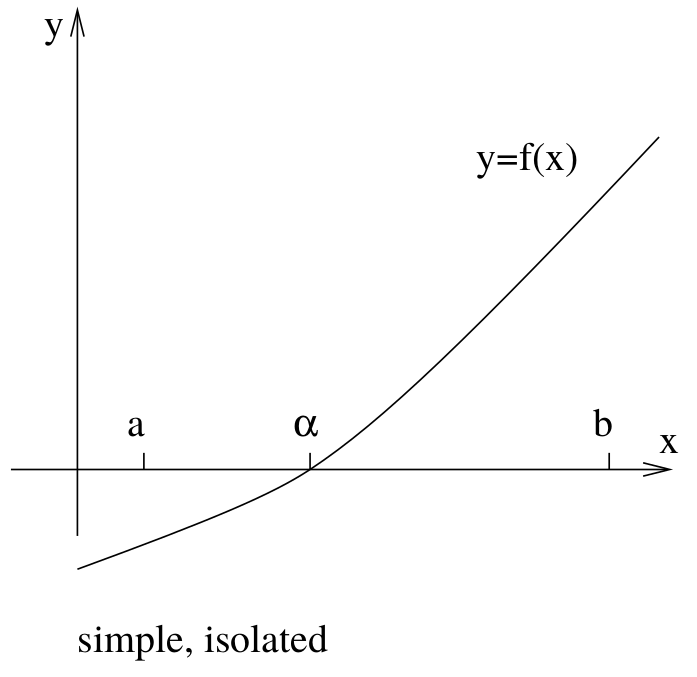
\includegraphics[width=1\linewidth]{img/7/7_1_1}
	\column{.5\linewidth}
		\centering   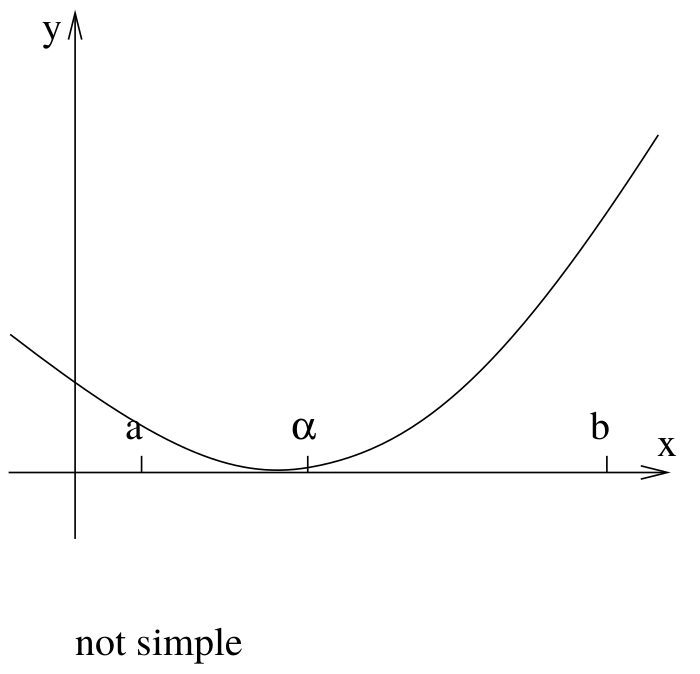
\includegraphics[width=1\linewidth]{img/7/7_1_2}
	\end{columns}
\end{frame}
%%%%%%%%%%%%%%%%
\begin{frame}{Wstęp}
	\centering 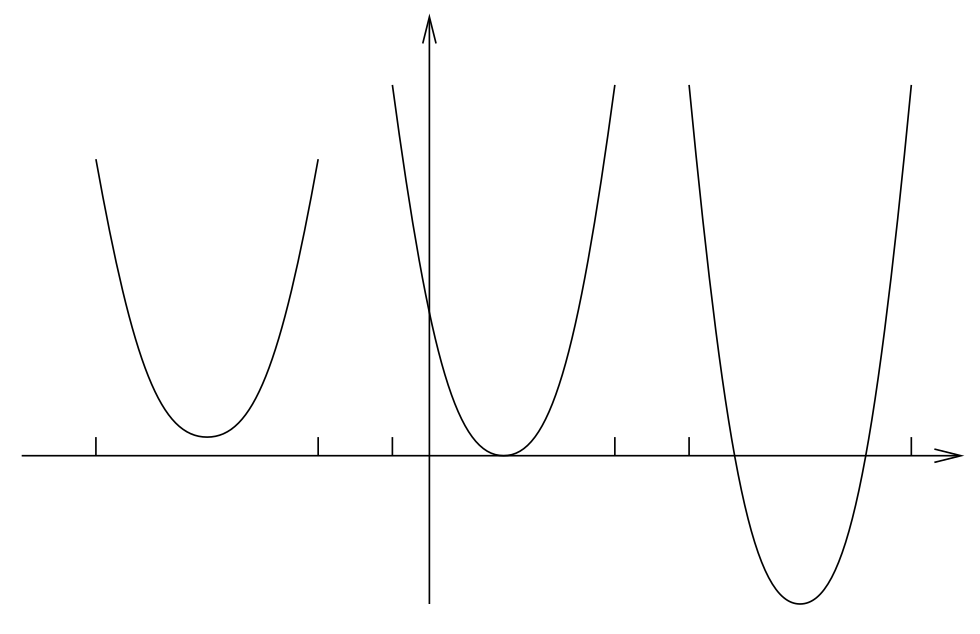
\includegraphics[width=1\linewidth]{img/7/7_1_3}
\end{frame}
%%%%%%%%%%%%%%%%
\begin{frame}{Wstęp}
	\begin{columns}
	\column{.5\linewidth}
		\centering   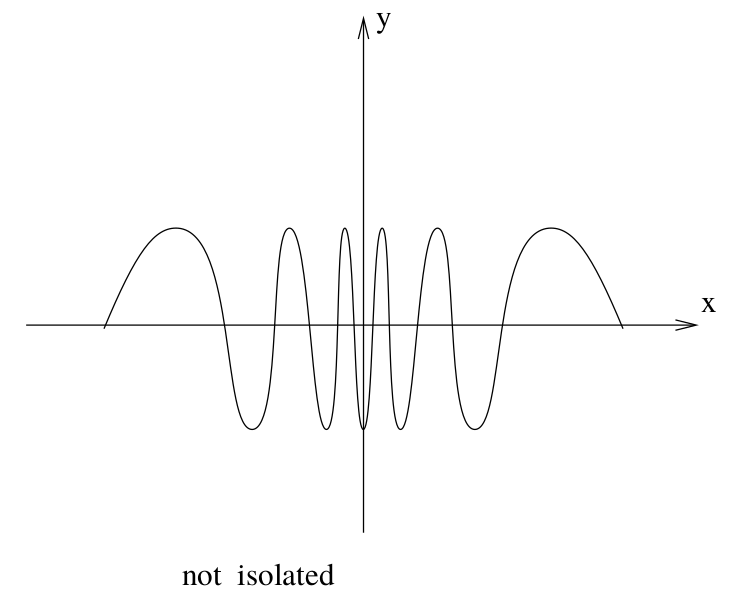
\includegraphics[width=1\linewidth]{img/7/7_1_4}
	\column{.5\linewidth}
		\centering   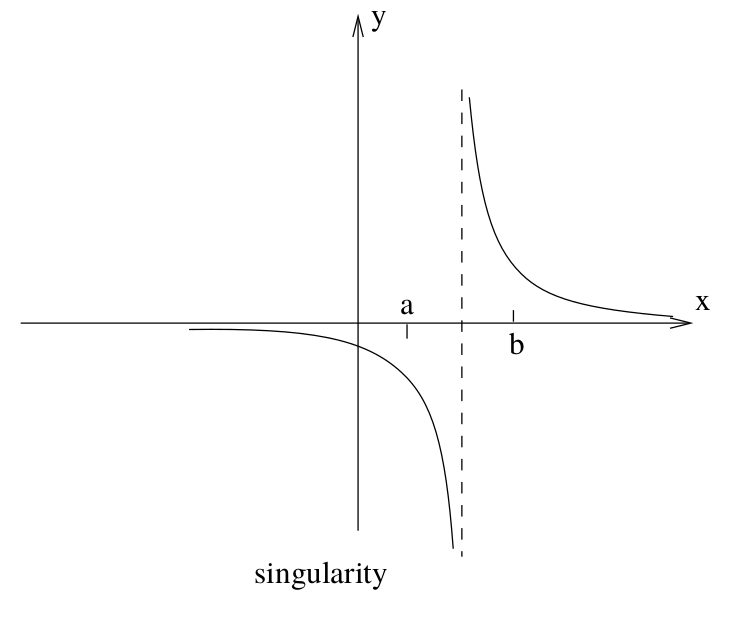
\includegraphics[width=1\linewidth]{img/7/7_1_5}
	\end{columns}
\end{frame}
%%%%%%%%%%%%%%%%
\begin{frame}{Wstęp}
	Należy więc:
	\begin{itemize}
		\item znać przebieg $f(x)$
		\item ``bracket a root''\newline
			  $\rightarrow$ przedział, w którym zmiana znaku funkcji,
		\item nie dopuszczać ``wyjść'' poza ustalony przedział.
		\item procedura szukania $\alpha$ {\bf nie może} być ``black box'' dla jej użytkownika!
	\end{itemize}
\end{frame}
%%%%%%%%%%%%%%%%
\begin{frame}{Wstęp}
	\centering   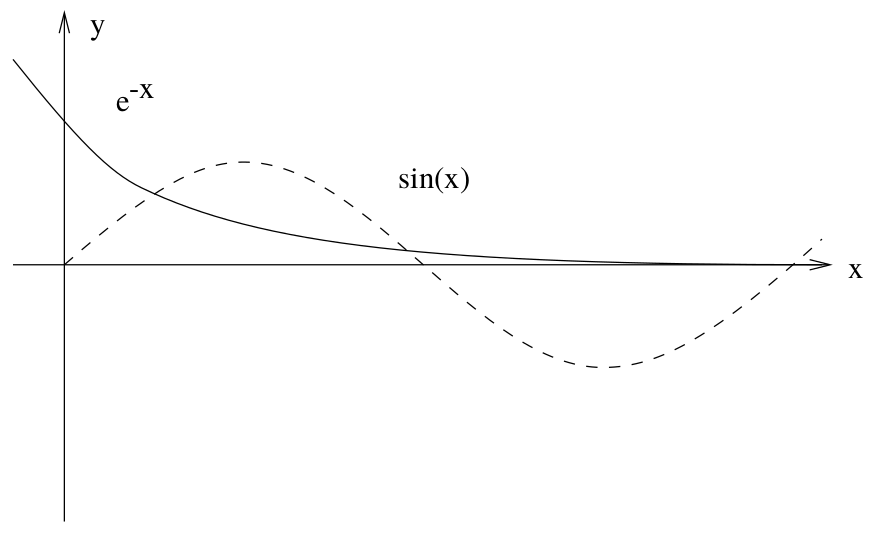
\includegraphics[width=1\linewidth]{img/7/7_1_6}
\end{frame}